
We've developed our methods by extending the basic intuition of \textit{OnlineCP}. Since dynamic tensor decomposition pursues shorter time factor updates, this will result low accuracy fitting when real-time data incomes. To optimize the speed accuracy problem, we'd like to trigger static decomposition like \textit{CP-ALS} while dynamic method like \textit{OnlineCP} is being done.

\subsection{\em OnlineCP-trigger}
\textbf{Detection Approach}: \textit{CP-ALS} activates whole temporal factor updates and enables high accuracy decomposition. Drastic data can be detected with image error norm and its ratio between every neighboring time frame is used to trigger \textit{CP-ALS} in this approach. The condition for triggering is when temporal ratio of error norm for incoming data exceeds threshold.

\begin{align*}
    threshold < \frac{\norm{\tilde{\chi}_{i+1}-\chi_{i+1}}}{\norm{\tilde{\chi}_{i}-\chi_{i}}}
\end{align*}

\begin{center}
	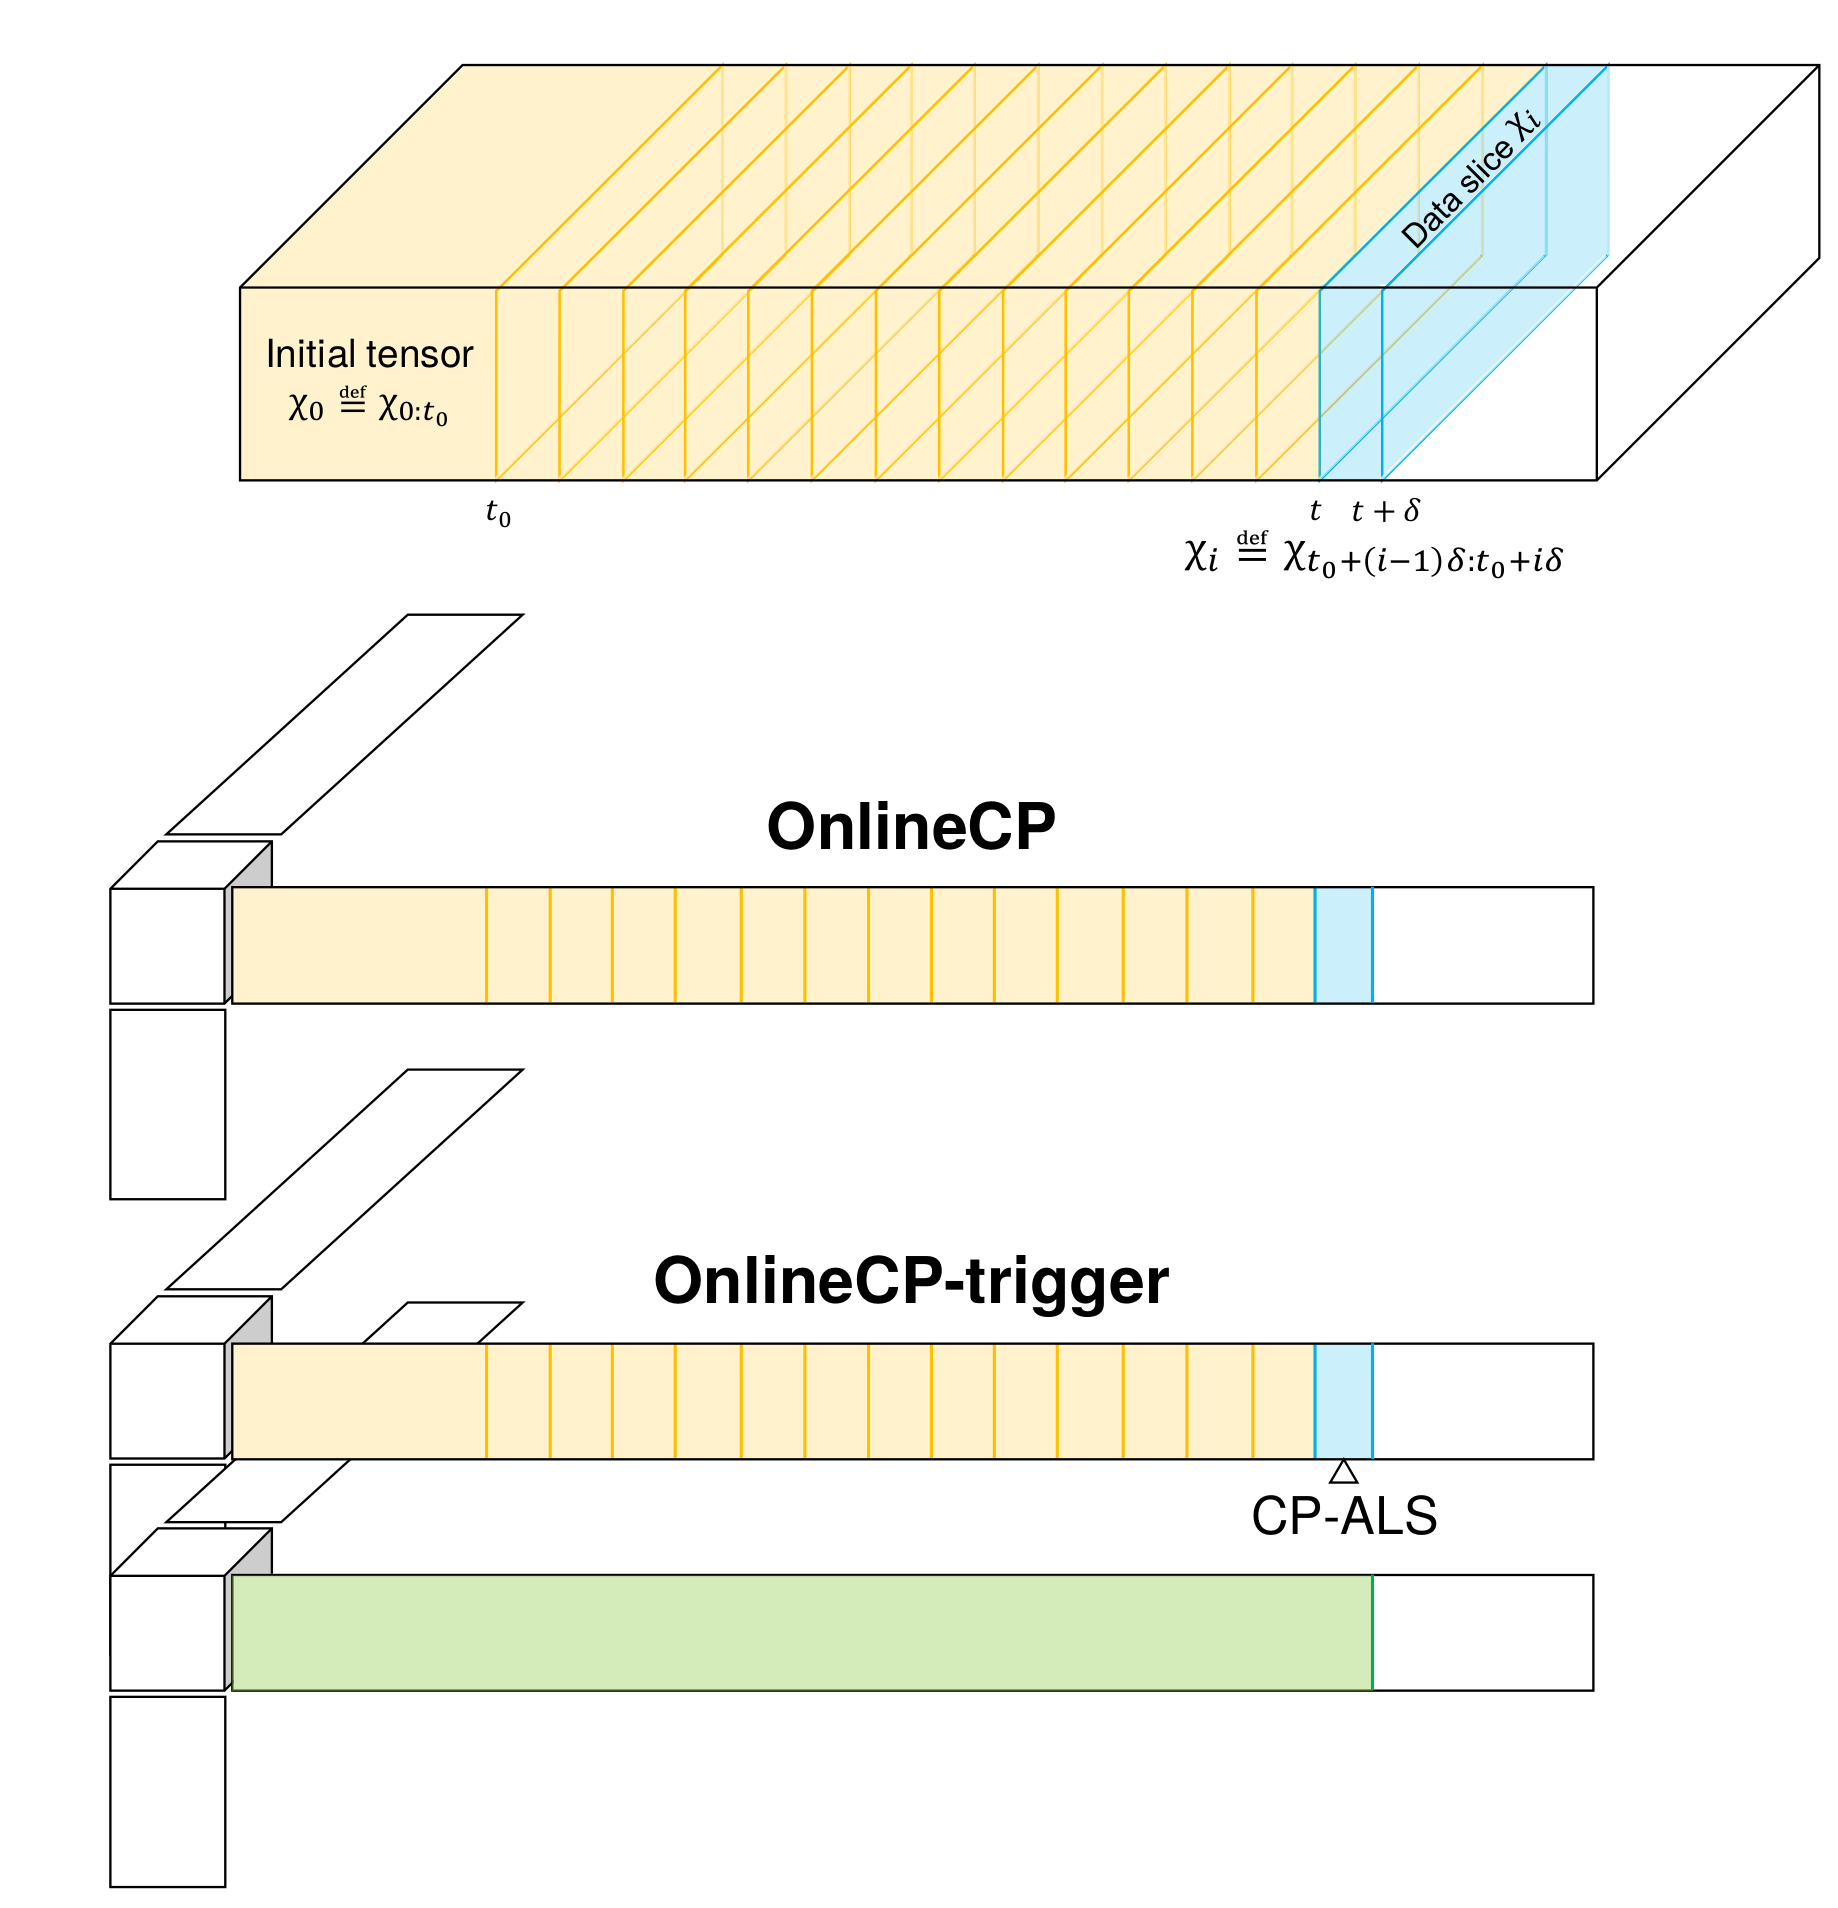
\includegraphics[width=0.8\textwidth]{FIG/OnlineCP-trigger.png}
\end{center}

\newpage
\subsection{\em OnlineCP-split}
\textbf{Split Approach}: trigger function in detection approach tells us sudden change in data. What if the incoming data may have a new theme unseen before? It implies that tensor separation and a new decomposition to start are needed. In this approach, we'd like to use the trigger function for splitting tensors to entirely different serial themes. (e.g. A, B, C, D)

\begin{center}
	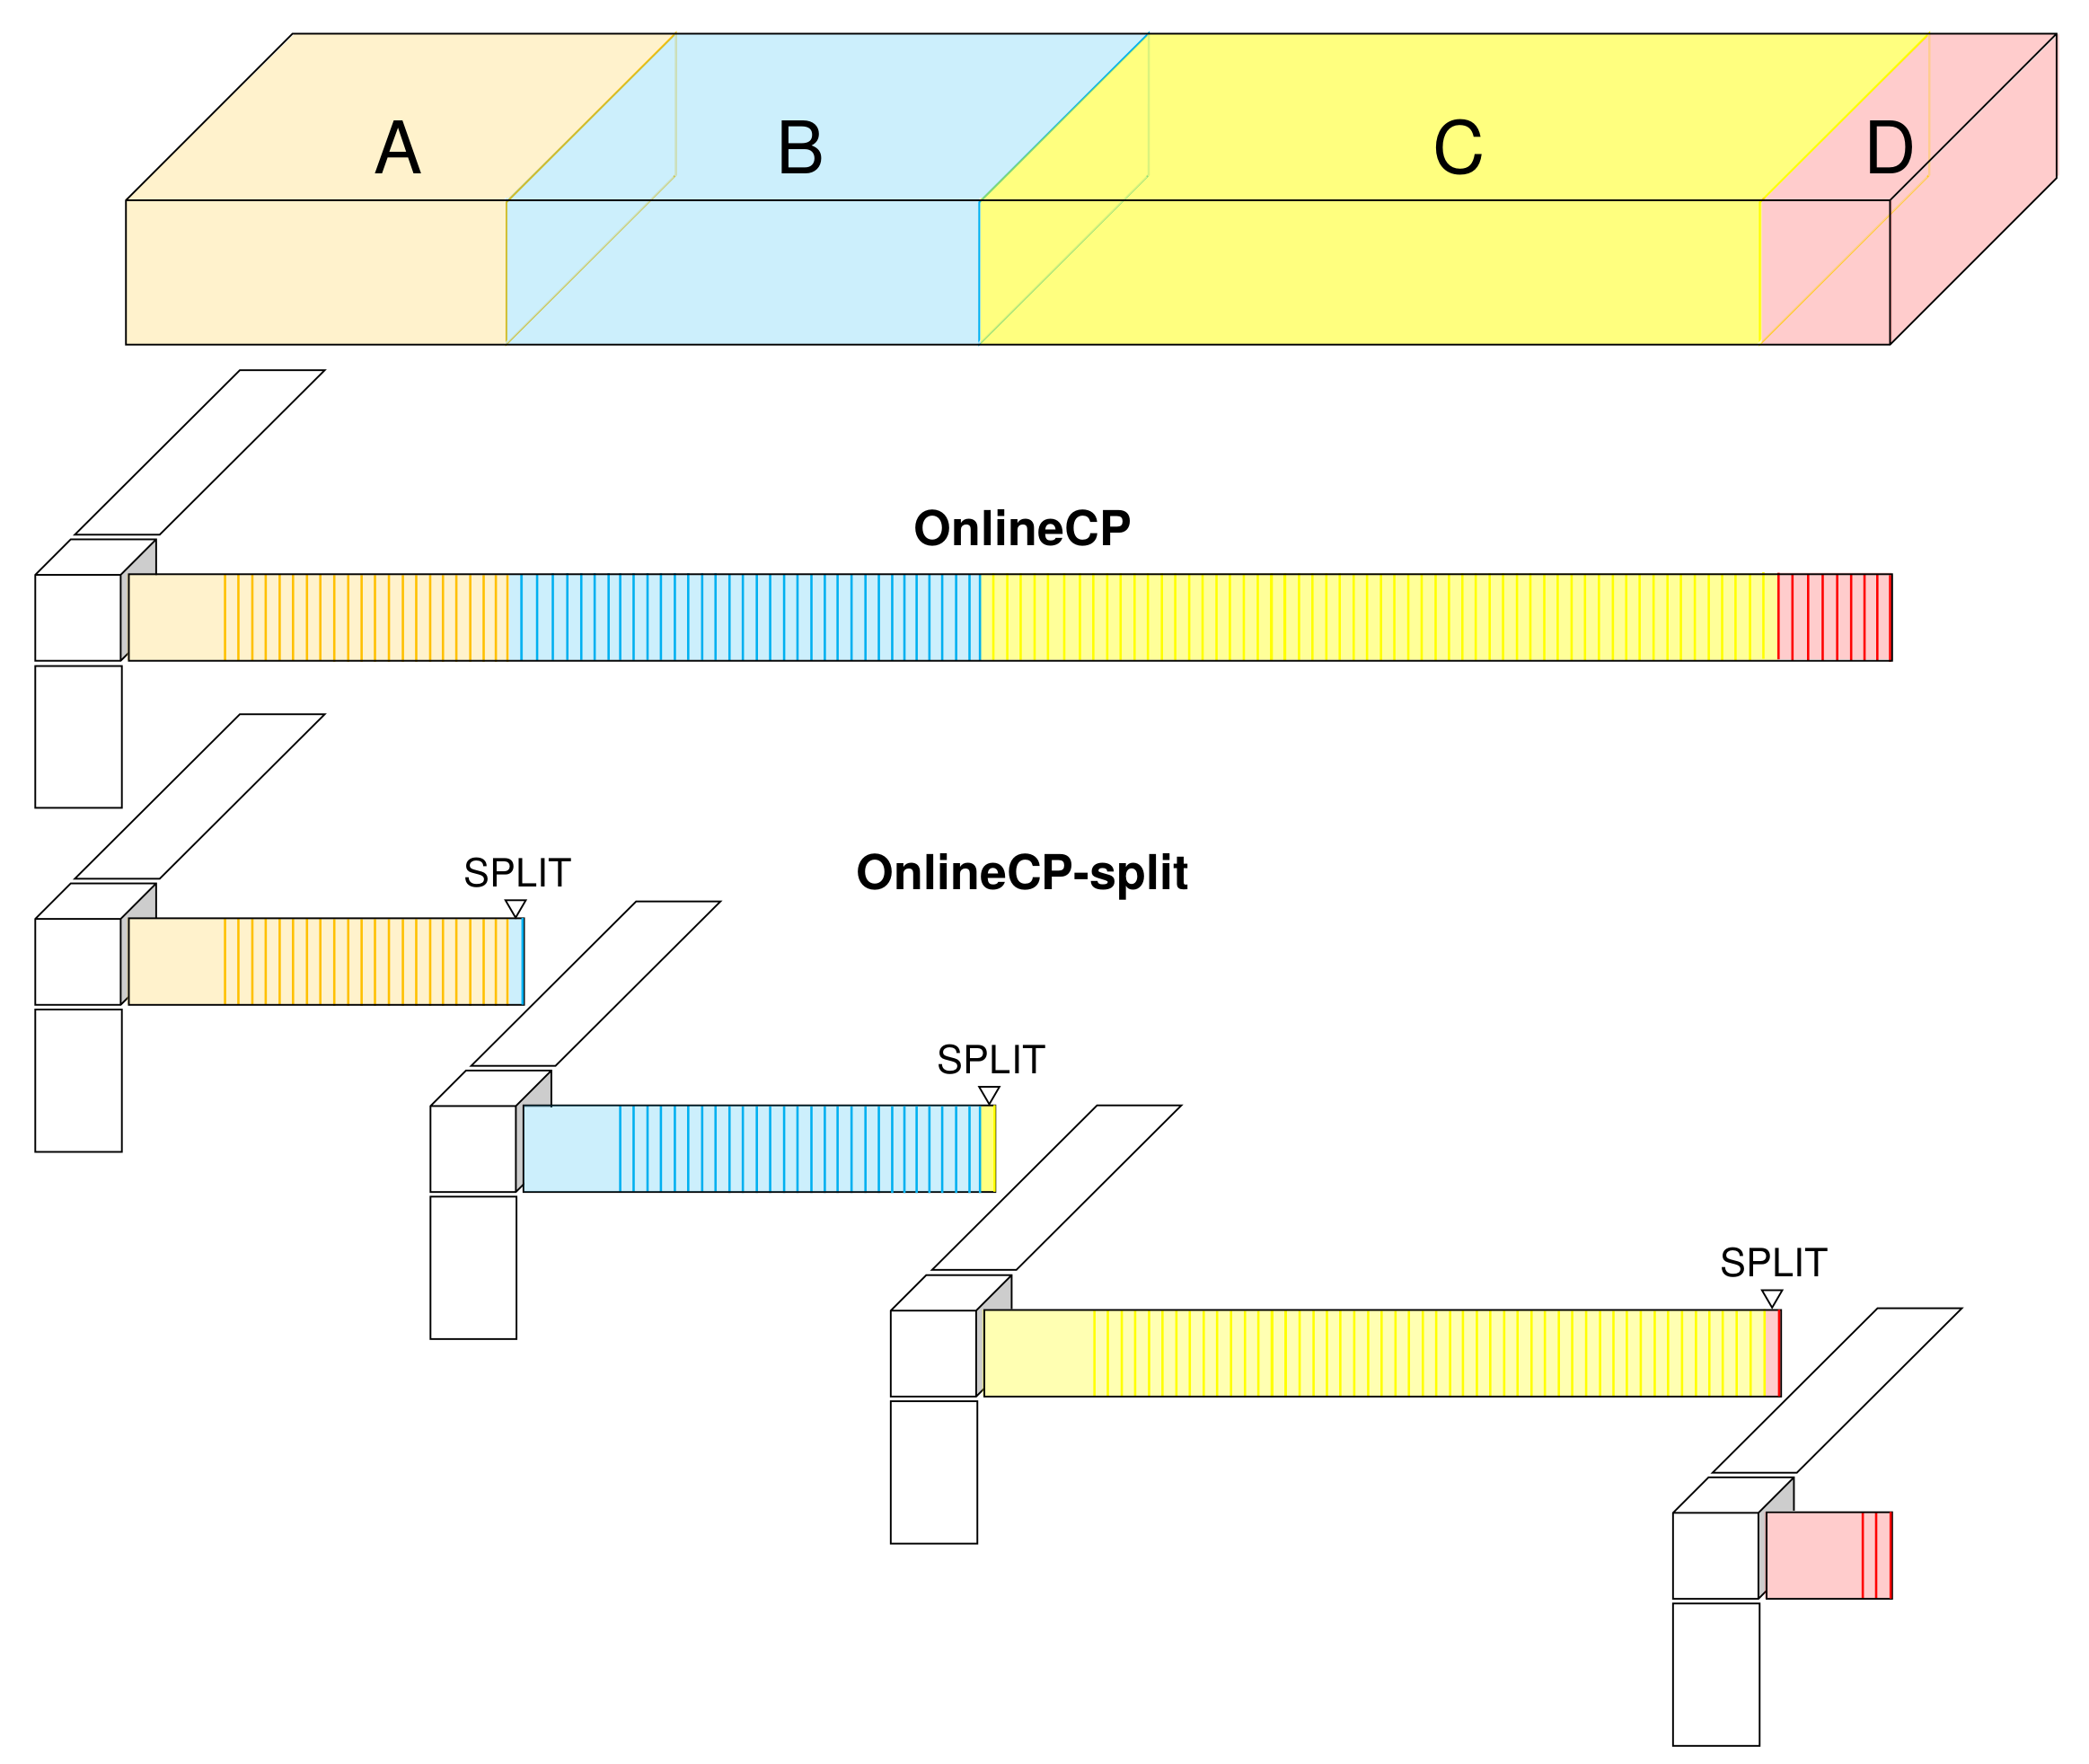
\includegraphics[width=1\textwidth]{FIG/OnlineCP-split.png}
\end{center}

\newpage
\subsection{\em OnlineCP-select}
\textbf{Selection Approach}: Similarly to split approach, trigger function makes a decision whether to split tensor or not to concatenate tensors behind with temporal factor updates. It allows to store the tensor efficiently; grouping tensors with similar themes and splitting them otherwise. (e.g. A, B, B’, C)

\begin{center}
	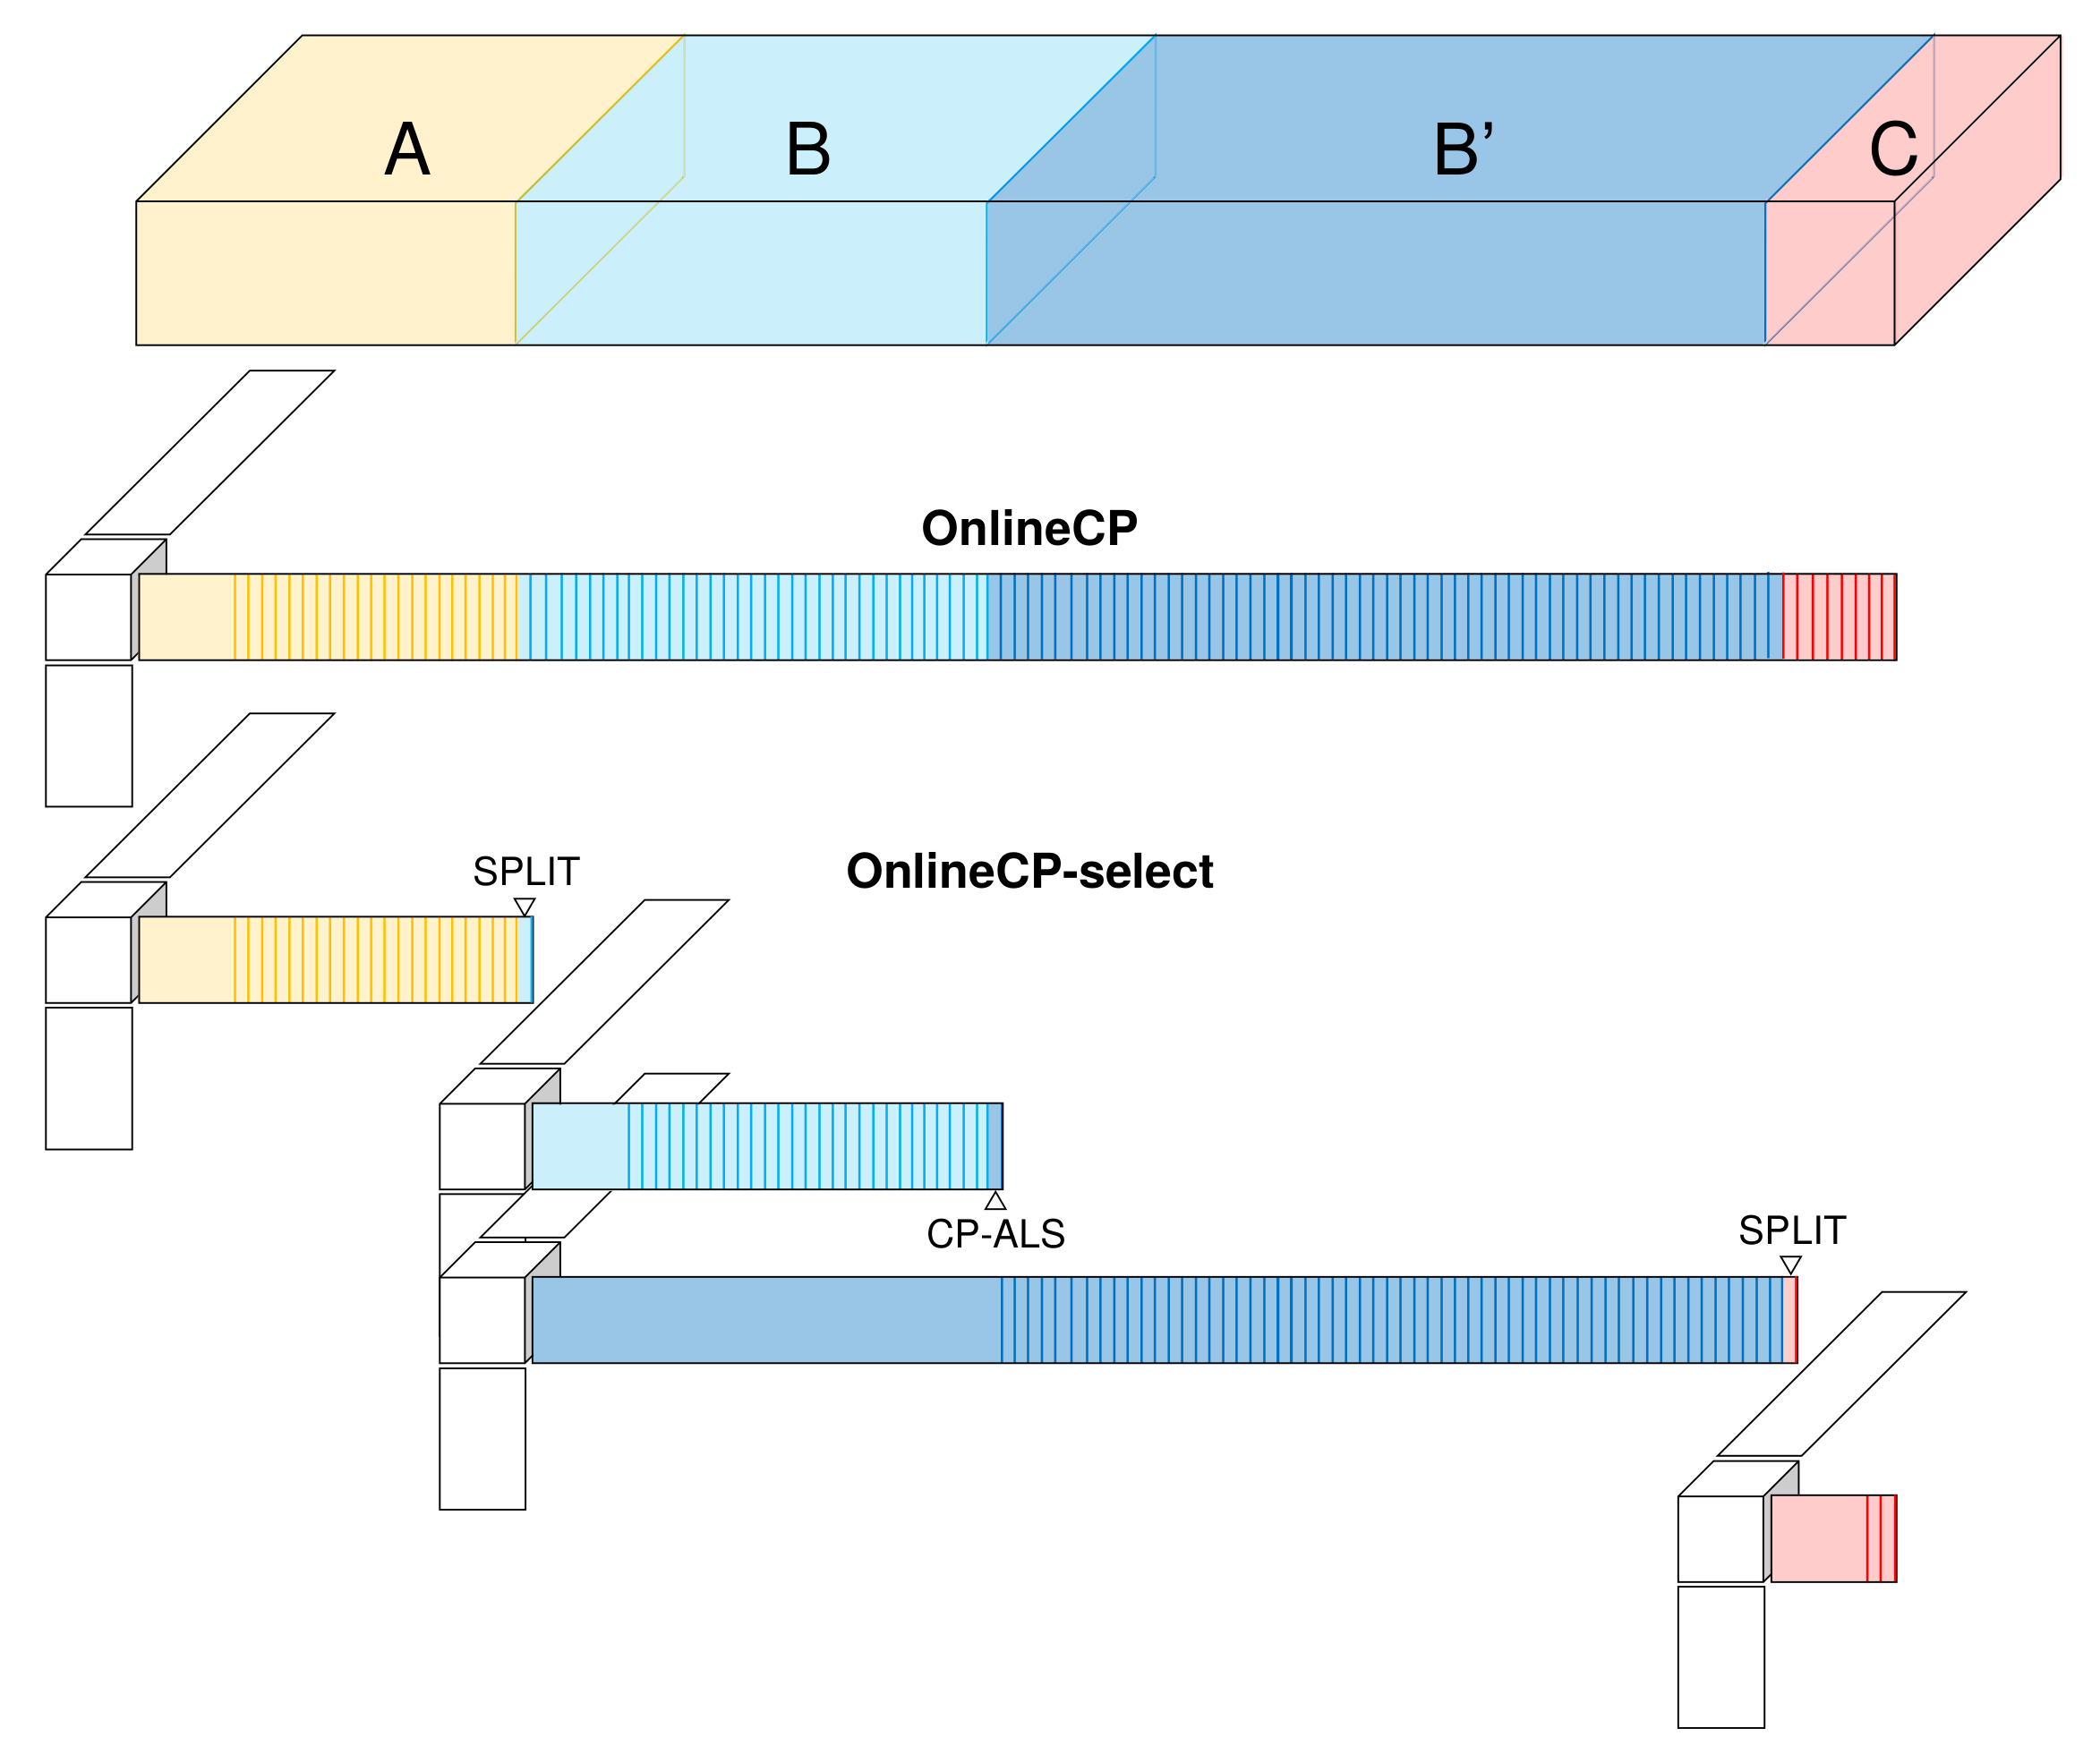
\includegraphics[width=1\textwidth]{FIG/OnlineCP-select.png}
\end{center}